\chapter{Modelling}
\label{ch:modelling}
\startchapter

The previous background chapter began with a high level overview of the game of Australian Rules Football and the coaches' role in providing feedback. This chapter formalises both of these concepts as models. This allows a more precise discussion and analysis of the concepts, and is an important step towards formalisms appropriate for mathematical analysis of the game.

The first research question (as defined in \secref{sec:questions}) asked whether team-level GPS analysis could provide useful information to sport researchers and practitioners beyond what they already know. In order to more precisely formulate this question, the field of information theory \cite{Shannon1948} is used to provide a formal definition of \textit{useful information} and to frame the role of sport data analysis systems within the larger domain of sport.

In order to prepare for automated analysis of spatio-temporal sport datasets, it is first necessary to establish terminology to describe the different kinds of spatio-temporal data. This takes the form of an abstract data model for spatio-temporal data. It is applied to describe the diversity of spatio-temporal datasets available in sport generally, as well as the AFL datasets used in this thesis.


\section{Model of Australian Rules Football}
\label{sec:model-of-afl}

The purpose of this section is to build a domain model of consistent terminology to describe Australian Rules Football. This allows linking formal reasoning about the game (e.g. mathematical models of game state) back to the somewhat looser jargon used by sport practitioners described in \secref{sec:information-available-to-coaches}.

% \todo{
%   Incorporate more details of game terms such as "behind" from old overview of game.
%   Refocus model here on describing the game rather than a simulation.
% }

Formally modelling games requires an understanding of the game \emph{state}. Decisions can then be strategically evaluated in terms of how they change this state. For example, in chess, the game state is the position of all the pieces on the board, which player has the next move, as well as other information needed to enforce the game rules, such as whether players still have the right to castle\footnote{Wikipedia Contributors, ``Board representation (chess)'' Available: \url{https://en.wikipedia.org/w/index.php?title=Board\_representation\_(chess)&oldid=880707099\#Requirements} Accessed:~2019-02-19}. In contrast to abstract strategy games such as chess in which the game state can be mathematically defined, fully describing the state of an Australian Rules Football game requires consideration of a large number of factors.

% In computer science, the strategy of an AI team can be thought of as a
% \emph{policy} that selects an \emph{action} as a function of the current
% \emph{state} of the game.
% From a formal perspective,  \emph{state} is important to comp
% In computer science, the strategy of an AI team can be thought of as a
% \emph{policy} that selects an \emph{action} as a function of the current
% \emph{state} of the game.

To capture aspects of the game relevant to describing the short-term and long-term state, the official \afl{} coaching manual \cite{afl2015coach} was manually mined for terminology, particularly chapter and section headings. These were then reassembled into a domain model as presented in \figref{fig:aflmodel}. The domain model is specified using the Unified Modelling Language (UML) standard maintained by the Object Management Group. Diamonds denote aggregation, the numbers near connectors represent multiplicity (e.g. a match has two teams, a team consists of multiple players), and triangles denote generalisation (e.g. disposals, possession and contact skills are types of individual skills, whereas problem solving, technical awareness and choice of technique are types of game sense). When mining the coaching manual, sections within a chapter were taken as an indicator of a possible relationship between terms in the section header and those in the chapter header. The development of the final model required an iterative process to improve the internal consistency of the terminology and incorporates minor refinements based on feedback from sport researchers\footnote{These were senior sport scientists on my current/former supervisory panel. This information is provided as an acknowledgement of their input, but should not be taken as a statement of expert validation of the final model.}.

\begin{landscape}

\begin{figure}[htbp]
\centering
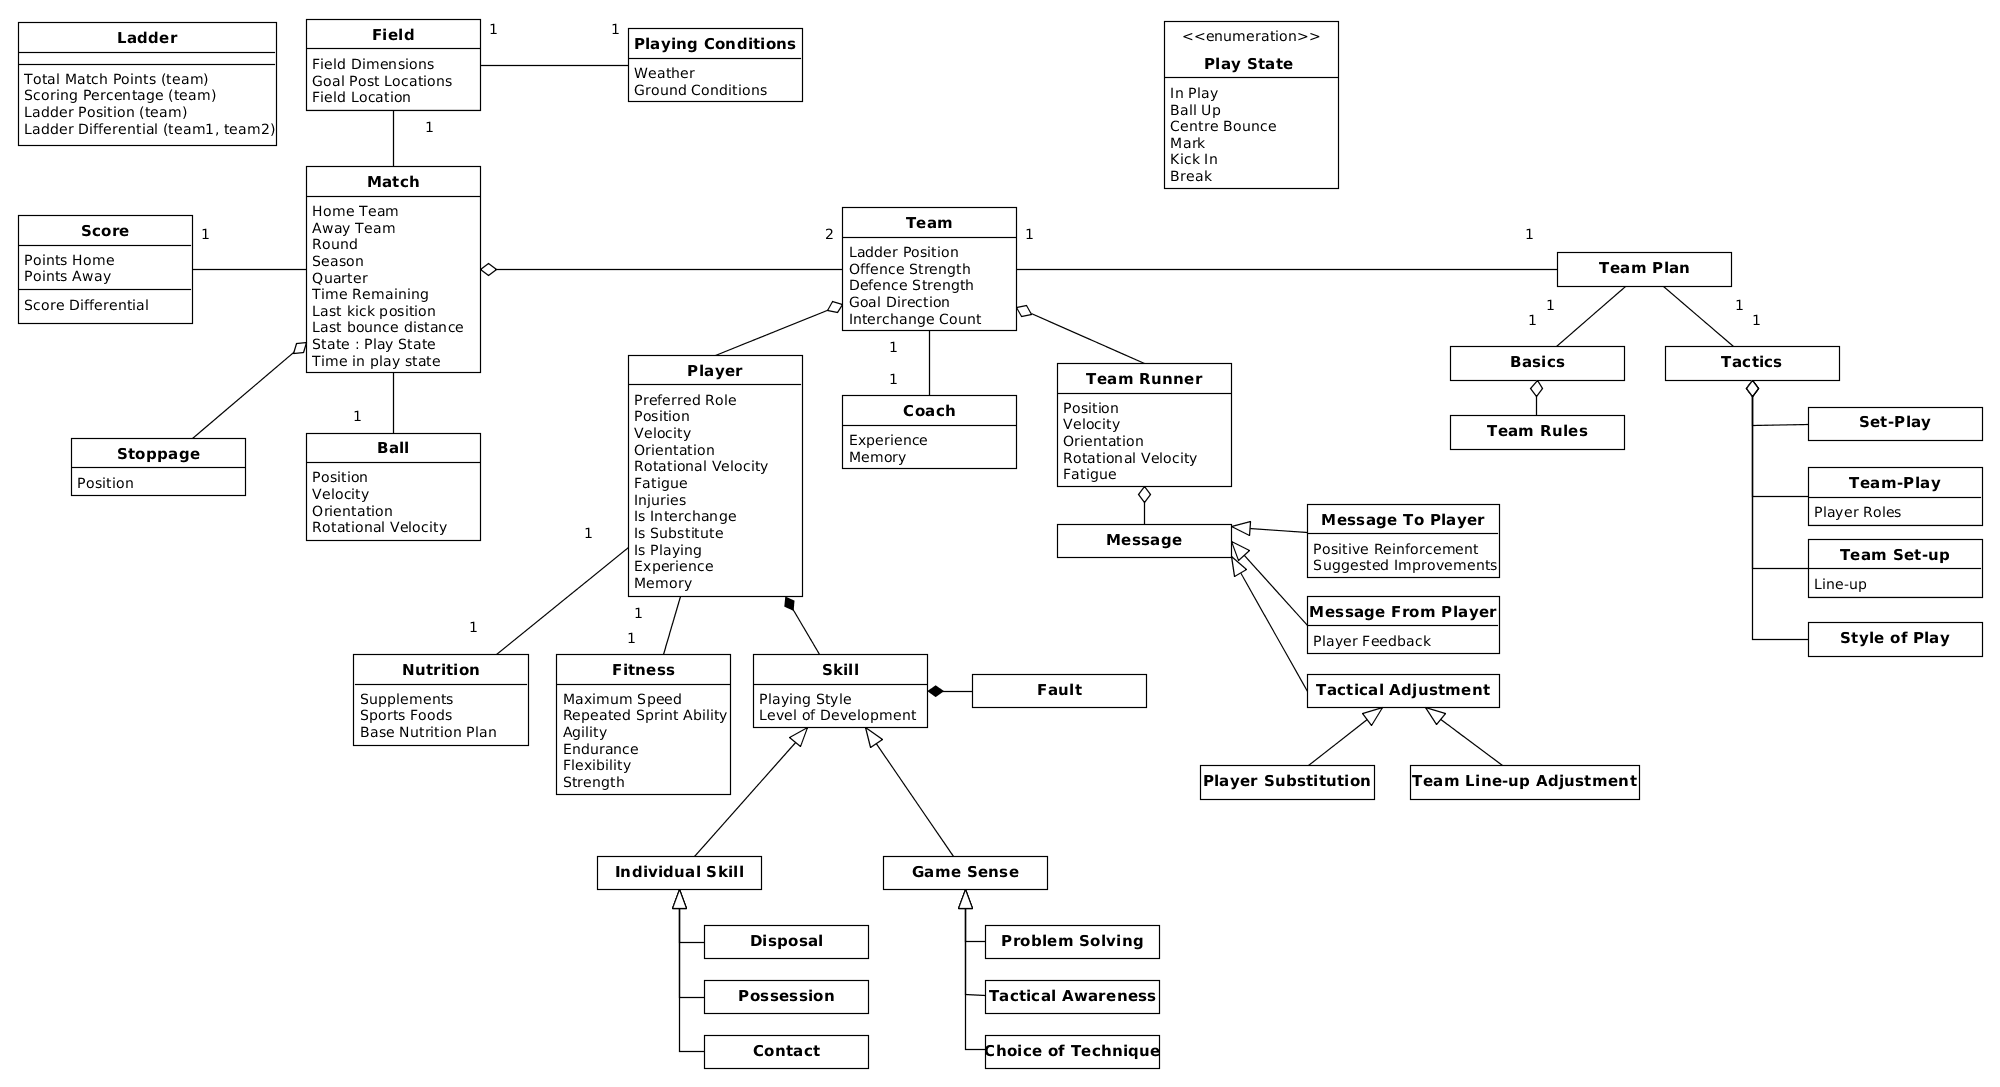
\includegraphics[width=\linewidth]{figs/model/afl_model_v3.png}
\caption{\afl{} Domain Model \label{fig:aflmodel}}
\end{figure}

\end{landscape}

% During game play, a coach is only allowed to communicate with their team
% by relaying messages via a team runner who runs out onto the field to
% provide a player a message from the coach. The rules state that runners
% are not allowed to directly instruct players; relayed messages should
% focus on providing players with feedback.\footnote{\url{http://www.afl.com.au/news/2014-06-18/crackdown-on-runners}}

This section will approximate the physical systems involved as rigid bodies. To avoid repetition of the parameters involved, let the \textit{kinetic state} of a rigid body be the set of variables required to completely describe the current state of the body within classical mechanics, \textit{viz.}, the position, velocity,
orientation, and rotational velocity. Forces are not included as part of the kinetic state, as forces are transient properties that only last as long as they are applied.

The information required to describe the current game state during a match\footnote{If modelling the game for the purpose of long-term decision making, then it would also be necessary to include additional information such as the team ladder position.} includes:

\begin{enumerate}
\item
  The score differential
  %The number of points scored by each team
\item
  The time remaining on the clock
\item
  The play state, for example, whether the game is in play, or has been
  paused by the umpires
\item
  Information needed by the umpires to enforce the laws of the game\footnote{For
  example, the player must bounce the ball at regular distance
  intervals, hence the distance since the last bounce is part of the
  game state.}
\item
  The kinetic state of the ball
\item
  The kinetic state of all players on the field (from both teams), and the team runners
\item
  The number of interchanges made by each team
\item
  The current weather and ground conditions
\item
  The level of fatigue each player is under
\item
  Any injuries sustained by players
\item
  The memory of players: what they have observed, and messages from the
  coach
\item
  The memory of the coaches: what they have observed, and messages from
  the players
\item
  The memory of the team runners: the current messages they are relaying
\end{enumerate}

As can be seen from the list of 13 game state components identified above (each in turn consisting of further state variables), it is non-trivial to precisely describe the state of an AFL game. Furthermore, some aspects, such as the state of information flows between coaches and players via team runners, impact upon the game\footnote{Peter Schwab (Brisbane Lions), 2013, ``In-Play Communication'' \url{http://www.aflcommunityclub.com.au/index.php?id=49&tx_ttnews\%5Btt_news\%5D=2768\&cHash=770d353c8665ecfac980dc8a70842de6} Accessed:~2019-02-19} but are not publicly recorded. In practice, it is necessary to approximate the game state to a simplified representation in order to permit formal reasoning about the game. In the past, formal models of \afl{} have simplified the game state by focusing solely on the location of the ball and which team has possession \cite{oshaughnessy_possession_2006, Jackson2016}, but this thesis aims to more closely approximate the true game state by using player position tracking data to incorporate the formation of team players on the field as part of the analysis.
